\documentclass[12pt, french]{article}

\usepackage{fancyhdr, fancybox, lastpage, makecell}
\usepackage[most]{tcolorbox}
\usepackage[a4paper, margin={0.3in, .75in}]{geometry}
\usepackage{wrapfig}
\pagestyle{fancy}
\renewcommand\headrulewidth{1pt}
\renewcommand\footrulewidth{1pt}
\fancyhf{}
\rhead{ \em{Zakaria Haouzan}}
\lhead[C]{\em{2ème année baccalauréat SM-X}}
\chead[C]{}
\rfoot[C]{}
\lfoot[R]{ \emph{Exercices Supplémentaires}}
\cfoot[]{\em{Page \thepage / \pageref{LastPage}}}


\newtcolorbox{Box2}[2][]{
                lower separated=false,
                colback=white,
colframe=white!20!black,fonttitle=\bfseries,
colbacktitle=white!30!gray,
coltitle=black,
enhanced,
attach boxed title to top left={yshift=-0.1in,xshift=0.15in},
title=#2,#1}


\begin{document}
\begin{center}
   \shadowbox {\bf{noyau énergie et masse (Supplémentaires)}}
\end{center}

\vspace{-0.2cm}
%%_________________________Exercice ! :"_________________________Exercice
%   \begin{center}
	   %\vspace{-0.6cm}
	%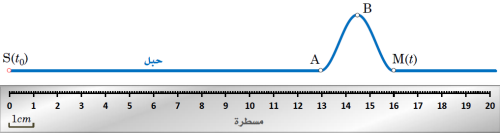
\includegraphics[width=0.6\textwidth ]{./img/Exercice01.png}
  %\end{center}



\begin{Box2}{Exercice 01 : la catastrophe nucléaire japonaise de fukushima le 11 mars 2011  }
	Les médias ayant couvert la catastrophe nucléaire japonaise de fukushima le 11 mars 2011, ont déclaré
que les taux de contamination radioactive des aliments a parfois dépassé de 10 fois les taux autorisés.
Par exemple l’activité de l’iode 131dans les épinards a varié entre 6100 Bq et 15020 Bq par
kilogramme. Au japon, les épinards sont considérés non contaminés, lorsque leur activité ne dépasse
pas 2000 Bq par kilogramme, comme niveau maximal admissible de contamination radioactive.

Le but de cet exercice est l’étude de la décroissance radioactive d’un échantillon d’épinard contaminé
par l’iode 131 radioactif. 

Données: La demi-vie de l’iode 131 $t_{1/2}=8jours$ ; $m(^{131}_{54}Xe)=130,8755u $ ; $m(^{131}_{54}X)=130,8770u $

\textbf{1. Etude du nucléide iode $^{313}_{53}I)$ } : 

\textbf{1.1. }La désintégration d’un noyau d’iode $^{313}_{53}I)$ , donne naissance à un noyau $^{313}_{54}Xe)$ . Ecrire l’équation modélisant cette désintégration, et préciser son type.

\textbf{1.2. }Calculer en MeV, l’énergie libérée par la désintégration d’un noyau d’iode 131.

\textbf{2. } Etude d’un échantillon d’épinard contaminé par de l’iode 131 : La mesure de l’activité d’un
échantillon d’épinard, pris d’une prairie proche du lieu de l’accident nucléaire, a donné la valeur 8000 Bq par kilogramme, à un instant considéré comme origine des temps.

\textbf{2.1. } Calculer le nombre $N_0$ de noyaux d’iode 131 radioactifs se trouvant dans l’échantillon
d’épinard étudié à l’origine des temps.

\textbf{2.2. } Déterminer, en jours, la plus petite durée nécessaires pour la décontamination des épinards
par l’iode 131.
\end{Box2}


\begin{Box2}{Exercice 02 : pile atomique}
	Dans une " pile atomique", une des réactions la plus courante est la suivante :$$^{235}_{92}U + ^1_0n \rightarrow ^{94}_{38}Sr + ^{140}_{Z}Xe + x.^1_0n$$

	\textbf{1. }Nommer cette réaction nucléaire.

	\textbf{2. } Déterminer, en les justifiant, les valeurs de Z et x.
	
	\textbf{3. } Calculer la perte de masse.
	
	\textbf{4. } Calculer, en joule, puis en MeV, l'énergie libérée par la fission d'un noyau d'uranium 235.
	
	\textbf{5. } Un réacteur utilise par jour en moyenne 3,0 kg d'uranium 235.
Calculer l'ordre de grandeur de l'énergie libérée par la fission de 3,0 kg d'uranium 235.

\textbf{Données : Masses des noyaux } $^{235}U = 234,993u$ ; $^{94}Sr=93,894u$ ; $^{140}Xe = 139,88909u$
\end{Box2}


\begin{Box2}{Exercice 03 :La Fusion nucléaire}
	L’équation d’une réaction deutérium-tritium est :$^{2}_{1}H + ^3_1H \rightarrow ^{4}_{2}He + ^1_0n$

	\textbf{1. } Exprimer l'énergie $\Delta{E}$ qui peut être libérée par cette réaction en fonction des énergies de masse $E_m(^A_ZX)$ des particules (ou des noyaux) qui interviennent.

	\textbf{2. } Exprimer la masse $m(^A_ZX)$ dun noyau $^A_ZX$ en fonction de $m_p$, $m_n$, Z, A et de l'énergie de liaison $E_L(^A_ZX)$. Pour la réaction de fusion envisagée, en déduire l'expression de $\Delta{E}$ en fonction des
énergies de liaison.

\textbf{3. } On donne les valeurs des énergies de liaison des noyaux suivants :
$E_L(^2_1H) = 2,224MeV$ ; $E_L(^3_1H) = 8,481MeV$ ; $E_L(^4_2He) = 28,29MeV$. Calculer numériquement la valeur de $\Delta{E}$.
\end{Box2}


\begin{Box2}{Exercice 04 :Etude d’un stimulateur cardiaque}
Le stimulateur cardiaque est un appareil médical introduit par chirurgie à l’intérieur du corps
humain qui souffre d’une insuffisance cardiaque Cet appareil fonctionne avec une batterie qui utilise
l’énergie nucléaire produit par la réaction de désintégration du noyau du plutonium $Pu$.
\begin{center}

\begin{tabular}{ |c|c|c|c|c| }
	\hline
Le noyau & $^A_ZX$ & $^{240}_{94}Pu$ & $^{238}_{94}Pu$ & $^{234}_{92}U$\\\hline
L’énergie de liaison EL en MeV &
28,285 &1813,008 &1800,827& 1778,142\\\hline
La demi- vie (ans)&
				  &  & 87,7&  \\\hline
\end{tabular}
\end{center}

\textbf{1. } Le plutonium a des isotopes tel que $^{240}_{94}Pu$ et $^{238}_{94}Pu$ . Déterminer le noyau le plus stable.

\textbf{2. } La désintégration du plutonium $^{238}_{94}Pu$ conduit à la formation du noyau d’uranium $^{234}_{92}U$ avec
émission d’une particule $^A_ZX$

\textbf{2.1 } Ecrire l’équation de désintégration du noyau du plutonium $^{238}_{94}Pu$ et déterminer la nature de la
particule émise.

\textbf{2.2 } Trouver en MeV l’énergie libérée $E_{lib}$ durant la désintégration d’un noyau du plutonium $^{238}_{94}Pu$.

\textbf{3. }A l’instant $t=0$ on introduit à un malade de 40 ans un stimulateur cardiaque. Le cœur du malade
fonctionne normalement jusqu’ à ce que l’activité du plutonium contenu dans le stimulateur
devient $a=0,7a_0$, avec $a_0$ l’activité a l’instant $t = 0$. Déterminer l’âge du malade lorsqu’on change
le stimulateur cardiaque
\end{Box2}


\begin{Box2}{Exercice 05 : centrale nucléaire}
Dans une centrale nucléaire, les noyaux d'uranium $^{235}_{92}U$ subissent la fission sous le choc d'un neutron
lent. Un des nombreux processus possibles conduit à la formation d'un noyau de lanthane $^{144}_{57}La$ ,d'un noyau de brome $^{88}_{35}Br$ et t de plusieurs neutrons.

\textbf{1. } Définissez l'énergie de liaison d'un noyau.

\textbf{2. } Donnez l'expression littérale qui permettra son calcul.

\textbf{3. } Calculez, en MeV, l'énergie de liaison d’un noyau $^{235}_{92}U$.

\textbf{4. } Calculez l’énergie de liaison par nucléon de ce noyau.

\textbf{5. } Ecrivez l’équation de la réaction de fission étudiée.

\textbf{6. } Exprimez l'énergie libérée par la fission d'un noyau $^{235}_{92}U$ en fonction des énergies de liaison par
nucléon du noyau père et des noyaux fils et calculez la valeur de cette énergie en MeV.

\textbf{7. } Dans le cœur de la centrale, de nombreuses autres réactions de fission du noyau $^{235}_{92}U$ se produisent. La perte de masse est, en moyenne, de 0,200 u par noyau.

\textbf{7.1. } Calculez, en MeV, l'énergie moyenne libérée par la fission d’un noyau. Ce résultat est-il en concordance avec celui de la question 6 ?

\textbf{7.2. }Calculez, en joule, l'énergie moyenne libérée par une mole de noyaux $^{235}_{92}U$

\textbf{Données :}
\begin{itemize}
	\item Célérité de la lumière dans le vide : $c = 2,998 . 10^8 m.s^{-1}$  
	\item Masse du noyau d’uranium 235 : $m( ^{235}_{92}U) = 235,0134u$ 

	\item Energies de liaison par nucléon : $E_l/A(^{144}_{57}La) = 8,28MeV/nucl$éon  ; $E_l/A(^{88}_{35}Br)$=$8,56MeV/nucl$éon
\end{itemize}
\end{Box2}


\begin{Box2}{Exercice 06 : la fission nucléaire}
Un tel sous-marin utilise comme combustible de l’uranium enrichi en isotope $^{235}_{92}U$ (cet isotope est fissile).

\textbf{1. } Donner la structure du noyau $^{235}_{92}U$.

\textbf{2. }Les noyaux d’uranium $^{235}_{92}U$ peuvent subir différentes fissions. La plus fréquente est donnée par l’équation suivante : $^{235}_{92}U + ^1_0n \rightarrow ^{94}_{38}Sr + ^{140}_{54}Xe + x.^1_0n$

\textbf{2.1. }Montrer que x = 2. Une justification soignée est demandée.

\textbf{2.2.} Montrer que l’énergie libérée par la fission, selon l’équation ci-dessus, d’un noyau
d’uranium 235 vaut $E_{lib} = 9,21.10^{-11}J$.

\textbf{3. }On suppose, pour simplifier, que les énergies libérées par toutes les réactions de fission sont
approximativement égales à celle calculée au 2.2.
Le réacteur fournit une puissance moyenne de 150 MW. On rappelle que $1W = 1J/s$.

\textbf{3.1.} Montrer qu’il se produit $5,15.10^{18}$ fissions par seconde.

\textbf{3.2.}  En déduire que la masse d’uranium consommée en 1s vaut $2,01 . 10^{-3} g$.

\textbf{4. } Un tel sous-marin est prévu pour naviguer pendant une durée de 2 mois. Quelle masse minimum d’uranium 235 devra-t-il embarquer pour assurer son approvisionnement en
énergie pendant cette durée?

m($^{235}_{92}U$) = 235,0439u ; m($^{94}_{38}Sr$) = 93,9154u  ; m($^{140}_{54}Xe$) = 139,9252u ;  Masse molaire de: M(U)=235g/mol
\end{Box2}


\begin{Box2}{Exercice 07 : La scintigraphie }
La scintigraphie est une technique d’investigation médicale qui permet l'observation de la glande
thyroïde. Un patient ingère pour cette observation une masse $m=1,31ng$ de l'isotope $^{131}_{53}I$ de l'iode qui
est radioactif de type $\beta^-$ 

$(t_{1/2}= 8,1 jours = 7.10^5s)$

\textbf{1. } Ecrire l'équation de la réaction de désintégration en justifiant.

\textbf{2. } Déterminer le nombre d'atomes radioactifs dans la dose ingérée.

\textbf{3. } On note $N_0$ le nombre de noyaux radioactifs à la date $t=0$. On note N le nombre de noyaux
radioactifs à la date t. Etablir la relation entre la constante radioactive $\lambda$ et le temps de demi-vie $t_{1/2}$, en précisant la signification de la demi-vie.

\textbf{4. } Définir l'activité d'un échantillon radioactif et établir la relation entre l'activité et N.

\textbf{5. } Calculer l'activité initiale de la dose ingérée.

\textbf{6. } Calculer le temps au bout duquel l'activité résiduelle est égale à 1,5\% de l'activité initiale.

\textbf{Données : } M(iode 131) = 131g/mol ; $N_A= 6.10^{23}mol^{-1}$; $^{51}Sb$ ; $_{52}Te$ ; $_{54}Xe$ ; $_{55}Cs$ ; $_{56}Ba$.
\end{Box2}

\begin{Box2}{Exercice 08 :radionucléide émetteur $\beta^-$
 }
Le cobalt $^{60}_{27}Co$ est un radionucléide émetteur $\beta^-$

\textbf{1. } Préciser la nature de la radioactivité $\beta^-$

\textbf{2. } Écrire l’équation de la réaction de désintégration du cobalt 60. Préciser les règles utilisées. On
donne $^{60}_{28}Ni$

\textbf{3. } L’activité A d’un échantillon est le nombre de désintégrations par seconde.

\textbf{3.1. } Sachant que cette activité A est proportionnelle au nombre N de noyaux non désintégrés qu’il contient, montrer que cette grandeur varie au cours du temps selon la loi : $ln(\frac{A_0}{A})=\lambda.t$.

\textbf{3.2. } Préciser le nom de la constante $\lambda$.

\textbf{4.} Calculer la demi-vie $t_{1/2}$ du cobalt 60, sachant qu'au bout d'un an, l'activité a diminué de 12\%.

\textbf{On donne : } $_{28}Ni$ ; $_{26}Fe$ ; $_{29}Cu$
\end{Box2}



\begin{Box2}{Exercice 09 :datation par l’Uranium-Plomb}

		Pour dater ou suivre l’évolution de quelques phénomènes naturels, les scientifiques font recours aux
méthodes et techniques diverses se basant essentiellement sur la loi de décroissance radioactive.
Parmi ces techniques : la technique de datation par l’Uranium-Plomb.
Données :Pour dater ou suivre l’évolution de quelques phénomènes naturels, les scientifiques font recours aux
méthodes et techniques diverses se basant essentiellement sur la loi de décroissance radioactive.
Parmi ces techniques : la technique de datation par l’Uranium-Plomb.

Données :
\begin{itemize}
	\item Masse du noyau d’Uranium 238 :238,00031 u || Masse du noyau du Plomb 206 : 205,92949 u
	\item Masse du proton: 1,00728 u || Masse du neutron : 1,00866 u
	\item L’unité de masse atomique : $1u = 931,5 Mev.c^{-2}$ ;
	\item Masse molaire de l’Uranium 238: $M(^{238}U) = 238 g.mol^{-1}$
	\item Masse molaire du Plomb 206 : $M(^{206}Pb) = 206 g.mol^{-1}$
	\item Energie de liaison par nucléon du Plomb 206 :E(Pb) = 7,87MeV/nucléon.
	\item  Demi-vie de l’Uranium 238 :$t_{1/2}= 4,5.10^9 ans$
		
\end{itemize}
Le nucléide Uranium 238 est radioactif, il se transforme en nucléide de Plomb par une succession
d’émissions de type $\alpha$ et $\beta^-$. 

On modélise ces transformations nucléaires par l’équation bilan suivante :$^{238}_{92}U \rightarrow ^{206}_{82}Pb + x.^0_{-1}e + y.^4_2He$

\textbf{1. Etude du noyau d’Uranium $^{238}_{92}U$ :}

\textbf{1. }Par application des lois de conservation, déterminer les valeurs de x et y signalés dans
l’équation bilan.

\textbf{1.2} Donner la composition du noyau d’Uranium 238.

\textbf{1.3} Calculer l’énergie de liaison par nucléon de l’Uranium 238, et vérifier que le noyau $^{206}_{82}Pb$ est plus stable que le noyau $^{238}_{92}U$.

\textbf{2. } Datation d’une roche métallique par la méthode d’Uranium-Plomb.

Le Plomb et l’Uranium se trouvent, avec des proportions différentes, dans les roches métalliques selon
leur date de formation.

On considère que la présence du plomb dans certaines roches métalliques est due seulement à la
désintégration spontanée de l’Uranium 238 au cours du temps. On dispose d’un échantillon d’une
roche métallique contenant à la date de sa formation, considérée comme origine des dates (t = 0), un
certain nombre de noyaux d’Uranium $^{238}_{92}U$ Cet échantillon métallique contient à une date t, une
masse $m_{ue}(t)=10g$ d’Uranium 238 et une masse $m_{Pb}(t) = 0,01 g$ de Plomb 206.

\textbf{2.1. } Montrer que l’expression de l’âge de la roche métallique est : 
$$t = \frac{t_{1/2}}{ln(2)}.ln(1+\frac{m_{Pb}(t) . M(^{238}U)}{m_U(t).M(^{206}Pb)})$$

\textbf{2.2 }Calculer t en années. 
\end{Box2}
	%\vspace{2cm}
%\begin{center}
   %\Large{ \em{Exercices Supplémentaires}}
%\end{center}


%\vspace{-0.7cm}
%%_________________________Exercice 5 : _________________________Exercice
%\begin{Box2}{Exercice 5 :Les ondes sonores }
%4
%\end{Box2}
%%_________________________Exercice 6 : _________________________Exercice
%\begin{Box2}{Exercice 6 : échographie}
%6
%\end{Box2}

\end{document}
